\chapter{Validação experimental, Simulação e Testes}
\label{chap:validacao}

\section{Introdução}
\label{validacao:sec:introducao}
\begin{comment}


    Referir que usámos a visualização em vez de métodos formais
\begin{comment}





\section{Requisitos do Sistema}
    artigo do sistema
    explicar que é uma simulação distribuída em vez de multithreaded (problemas de rede, etc)
    arquitetura do sistema
    engenharia de software

\end{comment}
 

\section{Construção do Sistema}
\label{validacao:sec:construcao}
\begin{comment}
- Explicação dos elementos do deploy - Makefile, Dockerfile, Docker-compose, 
> Explicar como funciona um Dockerfile
> "                         Dockercompose
> "             para que serve o Make.
- Explicar outra vez, mas resumidamente, a atualização da parte da visualização (não do estado no Node de visualização)
- Como dar deploy
\end{comment}

% Mudar palavras
Na implementação deste projeto foi necessário testar os \emph{Nodes} num contexto distribuído, no entanto, para que não seja necessário a execução de várias instâncias do programa em várias máquinas diferentes, fez-se uso de \emph{containers Docker} para se obter o mesmo efeito.

Além disso, o uso desta ferramenta provou-se útil na execução de múltiplas instâncias do programa, não apenas como ``Máquinas Virtuais'', de forma rápida e simples.

Na execução deste sistema para testes fez-se uso de três sistemas de construção, sendo estes ``docker'', ``docker-compose'' e ``Make'', cada um dependendo do anterior, por esta ordem.

Com o uso de estes sistemas de construção apenas é necessário executar o comando ``make run'' para executar um sistema com um \emph{Node} de visualização e um número arbitrário (mas definido num ficheiro ``docker-compose.yml'', ver capítulo seguinte) de \emph{containers} que executam o programa do \emph{Node}.

Como referido no capítulo anterior, o \emph{Node} de visualização faz uso de uma página \emph{Web} para demonstrar o estado (conhecido) do sistema. O endereço desta página depende do ficheiro ``Dockerfile'' (ver subsecção 
\ref{validacao:subsec:docker}
).


\subsection*{docker}
\label{validacao:subsec:docker}
Este sistema é usado na criação de \emph{docker containers} a partir da leitura de um ficheiro ``Dockerfile'', que descreve o processo de inicialização do \emph{container}, como que Sistema Operativo/imagem irá usar, a cópia de ficheiros para o \emph{container}, que comandos deve executar e por último que programa deverá executar.


% TODO: explicar melhor esta parte
Para a execução de \emph{Containers} que executam o programa do \emph{Node} foi usado o seguinte ``Dockerfile''.
\begin{lstlisting}[caption={``Dockerfile'' do \emph{Node}},language=C]
FROM golang # que sistema ou imagem ira usar, neste caso e usado a imagem ``golang''
WORKDIR /src  # em que diretorio, no container, os seguintes comandos irao ser executados
COPY . .
RUN go build -o node # compilacao do programa

# execucao da instancia, as variaveis de ambiente sao marcadas com $, no entanto serao descritas a sua origem de seguida
CMD ./node --address=$address --type=$type --link=$link --requests=$requests --visualization=$VIS_ADDRESS
\end{lstlisting}
 
Para a execução de \emph{Containers} que executam o programa do \emph{Node} foi usado o seguinte ``Dockerfile''.
\begin{lstlisting}[caption={``Dockerfile'' do \emph{Node}},language=C]
FROM golang # que sistema ou imagem ira usar, neste caso e usado a imagem ``golang''
WORKDIR /src  # em que diretorio, no container, os seguintes comandos irao ser executados
COPY . .

# compilacao do programa do \emph{Node} de visualizacao
RUN go build -o vis

# execucao da instancia do \emph{Node} de visualizacao
CMD ./vis

\end{lstlisting}

\subsection*{docker-compose}

Foram criadas várias tipologias de redes (por exemplo rede em Anel, Estrela, etc) para demonstrar e testar o diretório.
Estes exemplos estão no formato ``YML'', mais precisamente, no formato de um ficheiro ``docker-compose.yml'' para que este possa ser lido pelo programa ``docker-compose'', um \emph{script} que permite a execução de múltiplos \emph{containers} com apenas um ficheiro e um comando, sendo que este ficheiro faz uso de ficheiros ``Dockerfile''.

No entanto estes ficheiros apenas declaram os atributos de cada \emph{container}, como o nome, o endereço \acs{IP}, os \emph{Ports} que esta necessita para o funcionamento, e no contexto deste projeto, os atributos iniciais de cada \emph{Node}, como o ``Type'', o 
``Link'' e o enderço do \emph{Node} de visualização, visto que cada \emph{container} executará uma instância do programa, isto é, cada \emph{container} é um \emph{Node}. Os atributos do \emph{Node} são definidos usando as variáveis de sistema.


\begin{lstlisting}[caption={Ficheiro docker-compose.yml},language=C]
  # nome do container
  node_0:
    tty: true
    stdin_open: true

    # indicacao da localizacao do ficheiro Dockerfile
    build:
      context: ./src
      dockerfile: Dockerfile

    # definicao dos atributos do node como variaveis de ambiente
    environment:
      address: 127.0.0.1:8001
      type: 2 
      link: 127.0.0.1:8005
      VIS_ADDRESS: 127.0.0.1:8000/updateState
      requests: "true"

    # Ports necessarios para o funcionamento do Container
    ports:
      - "8001:8001"
    # Indicacao que este container sera executado na mesma rede que o Host, isto para que seja
    # possivel a realizacao de pedidos remotos atraves da visualizacao
    network_mode: host
\end{lstlisting}


\subsection*{Make}

% Melhorar frase introdutória
Na execução do sistema foi usado o sistema ``Make'', que executa comandos do Sistema Operativo. Para tal é necessário um ficheiro ``Makefile'' onde são descritos os vários comandos que serão executados ao executarmos o comando ``make''.

Por exemplo, caso se pretenda executar todo o sistema, apenas é necessário executar o comando ``make'' com o argumento (ou regra) ``start'', ou seja, ``make start'', invés de se executarem 7 comandos.


O ``Makefile'' usado neste projeto é o seguinte:

\begin{lstlisting}[caption={Ficheiro ``Makefile''}]

# constroi a imagem do \emph{Node} de visualizacao
build_viz:
	docker build -t vis ./visualization

# comeca o \emph{container} que executa o \emph{Node} de visualizacao
start_viz:
	-docker stop vis
	-docker rm vis
	docker run -it --net=host --env   address=:8000 --publish 8000:8000 --detach --name vis vis:latest

# comeca os \emph{containers} que executam os varios \emph{Nodes}
start_containers:
	-docker-compose stop
	docker-compose up --build --force-recreate -d

# Para a execucao de todos os \emph{containers} usados pelo sistema
stop_all:
	-docker stop vis
	-docker-compose stop


# Executa todas as regras necessarias para a execucao do sistema
run:
	$(MAKE) stop_all
	$(MAKE) start_viz
	$(MAKE) start_containers
\end{lstlisting}


\section{Interface de Visualização}
\label{validacao:sec:interface}
Para demonstrar o funcionamento e o estado do sistema, foi desenvolvida uma interface gráfica. Nesta secção serão descritos os componentes apresentados na interface de visualização.

\begin{figure}[!htb]
\centering
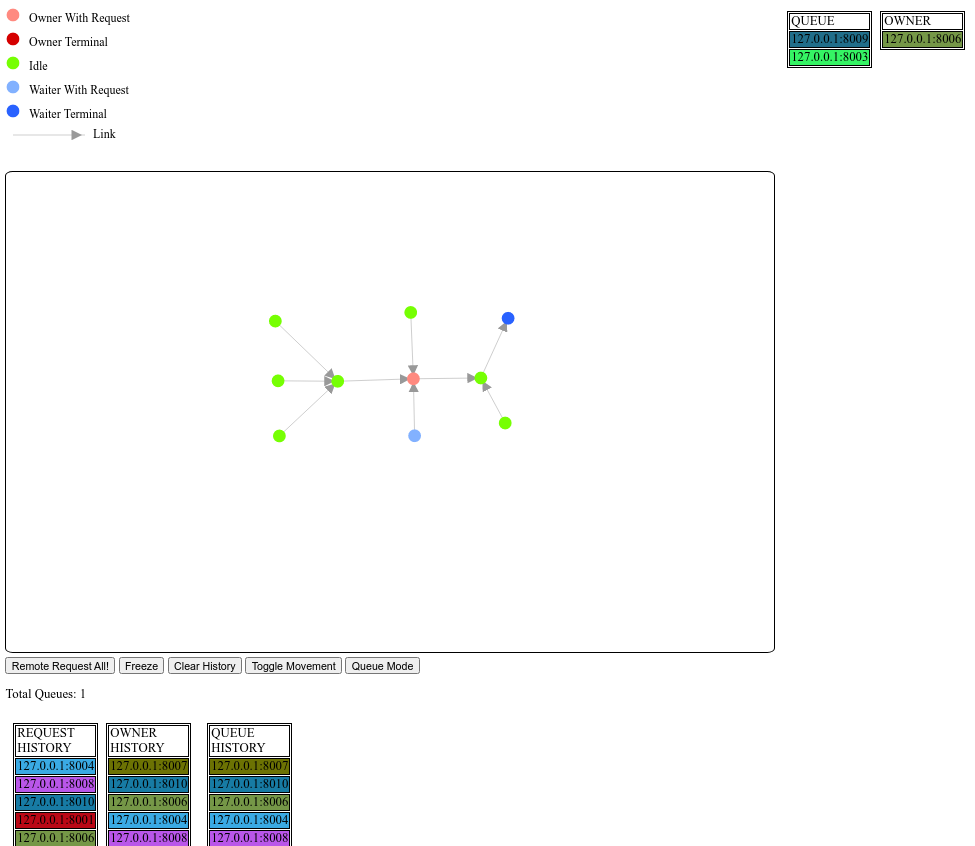
\includegraphics[width=300pt]{relatorio_overview.png}
\caption{Visão geral da interface.}
\end{figure}

Esta interface contém a informação sobre as duas estruturas de dados presentes no sistema, tabelas que contêm o histórico de vários eventos no sistema, e botões para interagir com o sistema e a visualização.

% TODO: Pôr uma introdução aqui.

\subsection*{Representação das Estruturas de Dados}
Na parte central da interface está apresentado um grafo, no qual os círculos representam os \emph{Nodes} e as setas representam os \emph{Links}. 
Também está presente uma etiqueta que indica qual o tipo do \emph{Node} corresponde à cor de um \emph{Node}.
As ligações (\emph{Links}) entre os \emph{Nodes} e as cores dos \emph{Nodes} são atualizadas dependendo do estado conhecido do sistema. 

Ou seja, há uma animação que vai evoluindo conforme o estado da rede conhecido pelo \emph{Node} de visualização, na qual é possível acompanhar que o comportamento de cada \emph{Node} altera a estado do rede.

É possível saber mais informação sobre cada \emph{Node}, deixando o ponteiro do rato por cima de um \emph{Node} e é possível forçar um \emph{Node} a realizar um pedido ao clicar neste.

Existe também o modo de filas/\emph{Queue}, que após pressionar o botão \emph{Queue Mode} (ver subsecção \ref{validacao:subsec:historico}
) as setas entre nós passam a demonstrar as ligações de filas/\emph{Queues} entre os \emph{Nodes}, ao invés das ligações do diretório.

Também estão apresentadas duas tabelas ao lado direito, com os títulos \emph{Queue} e \emph{Owner}, que representam a \emph{Queue} ``Principal'' e o atual \emph{Owner} conhecido.

\subsection*{Históricos}
\label{validacao:subsec:historico}
Na parte inferior da interface estão apresentadas 3 tabelas que contém informação sobre os seguintes históricos:
\begin{description}
    \item [\emph{Request History}] Histórico dos pedidos realizados pelos \emph{Nodes}.
    \item [\emph{Owner History}] Histórico dos \emph{Nodes} que tiveram o acesso ao objeto.
    \item [\emph{Queue History}] Histórico dos \emph{Nodes} da fila principal, isto é, a ordem da futura chegada do objeto aos \emph{Nodes}.
\end{description}

Esta informação não representa o estado da rede, mas é utilizada em testes. No entanto, o seu uso será descrito na secção \ref{validacao:sec:testes}.
% o grafo que representa o grafo distribuído/diretório e uma tabela que representa a fila/lista de espera ``Principal'' (que está diretamente ligada ao atual \emph{Owner}), 

\subsection*{Botões}
Na interface estão disponíveis 5 botões diferentes que permitem a iteração com o sistema e a visualização. A funcionalidade de cada botão é a seguinte:
\begin{description}
    \item [Remote Request All] - Força todos os \emph{Nodes} conhecidos a realizarem pedidos. Usado para testes.
    \item [Freeze] - Para qualquer atualização da interface de visualização.
    \item [Clear History] - Apaga as tabelas de histórico.
    \item [Toggle Movement] - Bloqueia o movimento de todos os círculos que representam os \emph{Nodes} no grafo.
    \item [Queue Mode] - Ativa o modo de demonstração das filas.

\end{description}

\section{Testes}
\label{validacao:sec:testes}
%TODO: explicar o quão diferente é a única implementação conhecida
No desenvolvimento foi necessário testar a implementação e também provar o seu bom funcionamento, no entanto não foi possível fazer-se uso de métodos formais de prova deste sistema, nem de comparar esta implementação com outra existente, visto que, a implementação feita no decorrer deste projeto é muito diferente da única conhecida.
						%mudar "histórico VVVVV"
Ainda assim é possível testar o bom funcionamento do sistema fazendo o uso dos elementos presentes na interface gráfica disponibilizada.
% Talvez especificar todas as questões de bom funcionamento?

Nem todos os elementos da visualização estão atualizados em qualquer momento, por exemplo, ambos o grafo e as tabelas da fila ``Principal'' podem estar em desacordo com o estado real do diretório, pois ambos dependem da última informação conhecida pelo \emph{Node} de visualização, que pode ter um \emph{Delay} causado tanto pela atualização (ou \emph{Refresh Rate}) da interface, a rede usada para comunicação, a sincronização da chegada de informação, etc., mas ao longo do decorrer do sistema, estes serão corrigidos.


É possível, na demonstração gráfica do diretório (o grafo) ser mostrado um estado impossível, como, por exemplo, mostrar vários \emph{Owners}, sendo que na realidade só existe um único, ou uma ligação em falta, porém, a implementação estaria errada caso um \emph{Node} se ligar a um \emph{Node} que previamente não era seu vizinho, pois, como definido no protocolo estudado, os vizinhos de um \emph{Node} são sempre as mesmos, apenas as ligações entre estes é que são alteradas (invertidas).

No entanto, o uso mais indicado do grafo e das tabelas da fila e atual \emph{Owner} é de visualização e demonstração de como funciona o sistema/protocolo, e não como prova, devido aos problemas de atualização presentes. 

Para uma evidência mais forte, fez-se uso das 3 tabelas dos históricos. 
Como referido anteriormente, a tabela \emph{Queue History} mostra o histórico dos \emph{Nodes} que entraram na fila ``Principal'', e a passagem do acesso ao objeto tem de seguir a ordem dessa fila, e a ordem por onde circula o objeto é mostrado na tabela \emph{Owner History}, logo, caso as tabelas \emph{Queue History} e \emph{Owner History} demonstrem os \emph{Nodes} com ordens diferentes, o sistema está errado.

A tabela \emph{Request History} tem apenas demonstra que a ordem pela qual os \emph{Nodes} realizam pedidos ou que a ordem que \emph{Node} de visualização recebe a atualização de que esses \emph{Nodes} realizaram pedidos pode ser diferente da ordem na file ``Principal''.



\section{Conclusões}
\label{validacao:sec:conclusoes}
Neste capítulo foi feita uma descrição do funcionamento do sistema usado para a visualização e teste do programa \emph{Node}, sendo este um dos pontos de maior interesse deste projeto. O uso de ferramentas de construção provou-se útil na execução do sistema num contexto distribuído, de forma fácil, rápida, que pode ser usada para replicar a construção deste sem ter conhecimento da implementação do programa. Foi também uma explicação do funcionamento da interface e como se testou o sistema e demonstrou o bom funcionamento deste.
